\chapter{Derivation of Parasite Clearance Times}
\section{Overview}
The client specified that the endpoint of primary importance is PC90, the time to achieve a reduction of the parasitaemia by 90\% of baseline level. 

As a first attempt at deriving estimates of PC90 from the data, simple linear polynomial fits to the logarithm of the parasite count with time from first dose were investigated (actually log(1+parct)).

It was found that a cubic was the most suitable model if we include the data only up to the first 0 parasite count. For some patients where the parasite count drops quickly to 0. A fit that includes the subsequent run of 0s would pull the cubic fit away from the most sensible estimate of PC90. It is more suitable for the purpose of estimating PC90 to only model the drop in the count to 0 using a simple cubic model. 

Figure \ref{cubics} shows the cubic fits to the log parasite count for the 43 subjects treated. The horizontal dotted line on the plots shows the PC90 level i.e. where the parasite count has fallen to 10\% of its initial value. The value of PC90 i.e. the time t at which the parasite count has fallen to 10\% was found by least-squares i.e. using the \texttt{optimize} function in R to minimise:
$$[log(1+0.1P_0)-\beta_0-\beta_1t-\beta_2t^2-\beta_3t^3]^2$$
where $P_0$ is the pre-treatment parasite count, $t$ is the time from first dose and $\beta_i$ are the fitted coefficients for the models for each of the 43 patients. Table \ref{pc90} shows the values of PC90 derived from the cubic fit to the parasite count by centre, sex and treatment.
\begin{sidewaysfigure}[p]
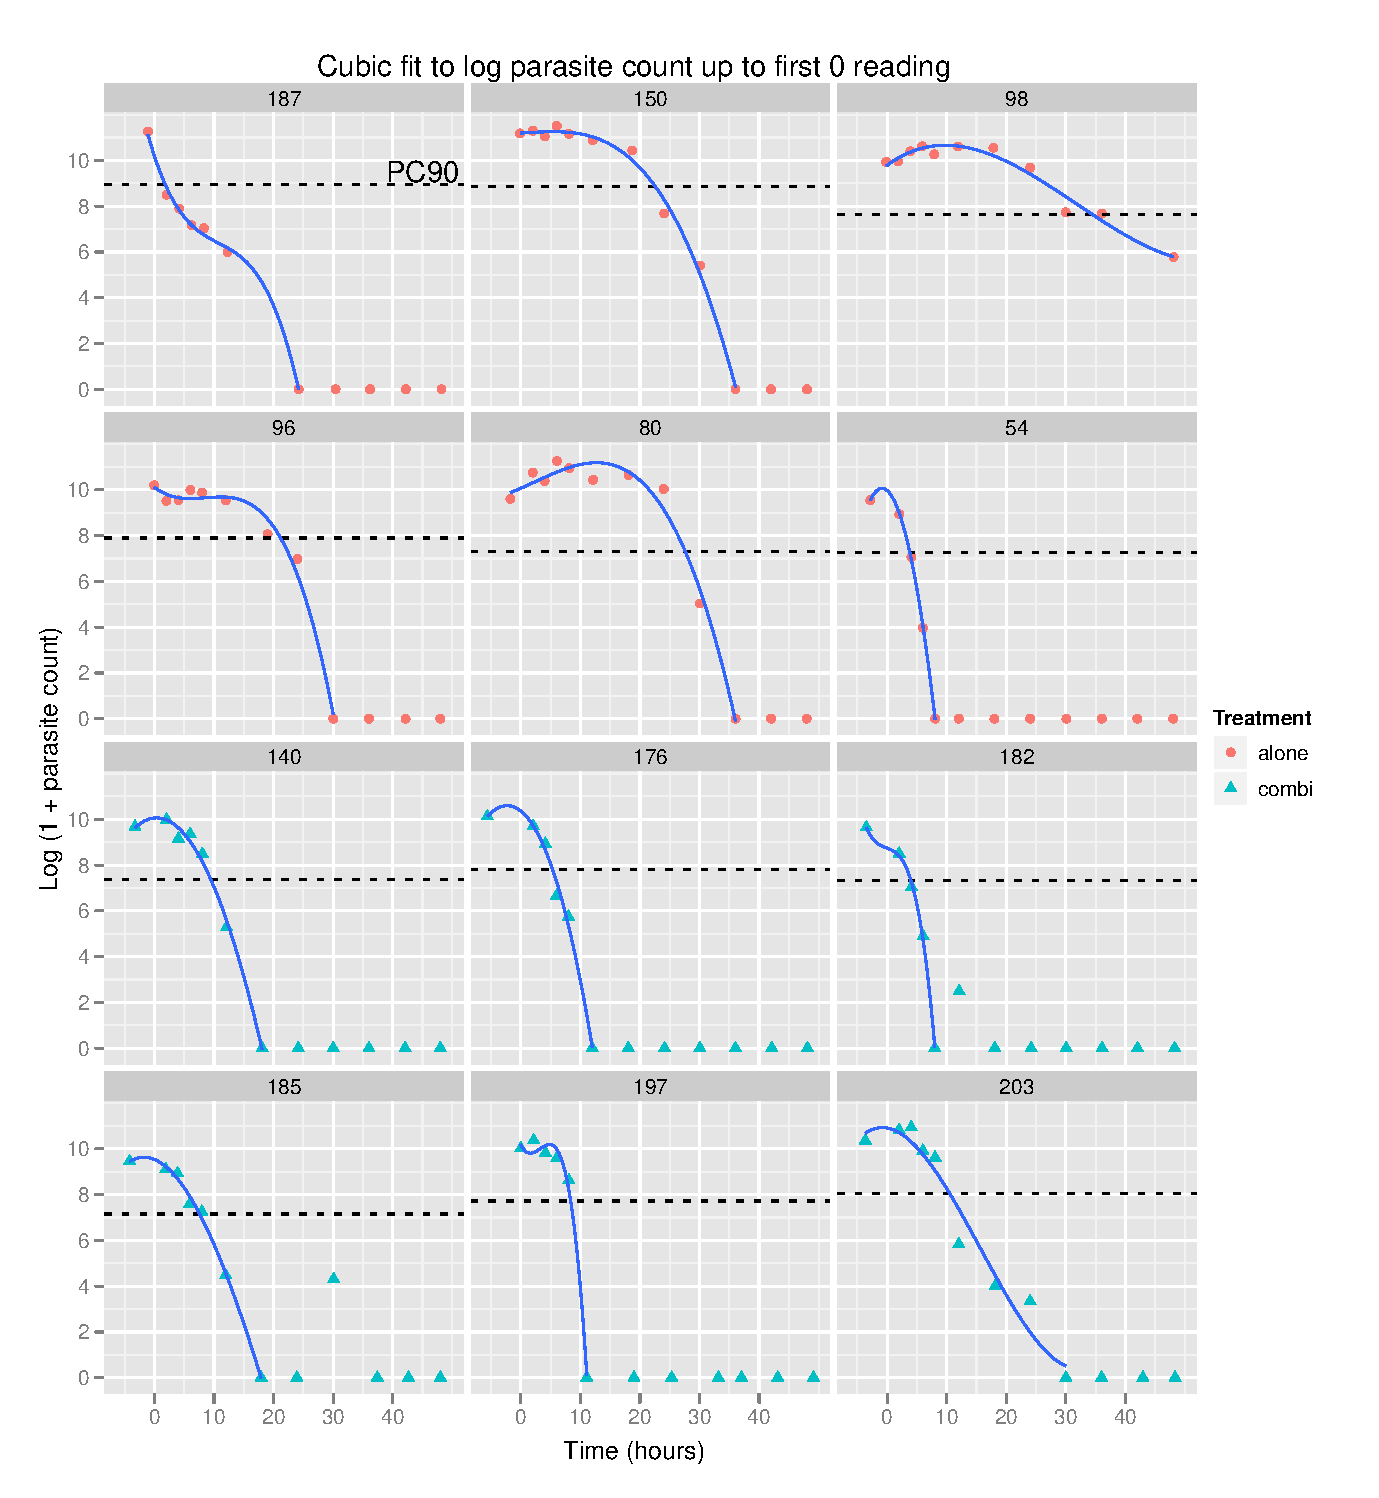
\includegraphics[scale=0.8]{cubics.eps} 
\caption{Cubic fits to log parasite count vs. time from first dose for 43 subjects treated}\label{cubics}
\end{sidewaysfigure}
\begin{table}[h]
\centering
\caption{Derived PC90 values}\label{pc90}
\begin{tabular}{|cc|c|c|}
\hline
&&\multicolumn{2}{c|}{Treatment}\\
Centre&Sex&A&B\\\hline
\multirow{2}{*}{001}&M&$\begin{array}{c}3.8,\ 27.9,\ 34.3,\  9.8,\\5.0,\  0.8,\ 28.9,\  4.7\end{array}$&$\begin{array}{c}9.5,\  5.3,\  7.7,\\23.5,\  9.4,\  8.1\end{array}$\\\cline{2-4}
&F&$\begin{array}{c}21.1,\ 23.2,\\22.5,\ 47.2\end{array}$&$\begin{array}{c}4.2,\ 8.6 ,\ 9.4,\\0.9,\ 8.6,\ 12.9\end{array}$\\\hline
\multirow{2}{*}{002}&M&$\begin{array}{c}4.5,\ 2.1,\\20.6,\ 29.1\end{array}$&$\begin{array}{c}19.3,\ 10.0,\\15.6,\ 8.9\end{array}$\\\cline{2-4}
&F&$\begin{array}{c}20.1,\ 2.2,\ 24.0,\ 28.7,\\5.0,\ 22.2,\ 23.7\end{array}$&$\begin{array}{c}15.4,\  8.4,\\5.9,\ 6.3\end{array}$\\\hline
\end{tabular}
\end{table}
\subsection{PC90 ANOVA} 
3-way ANOVA with interactions was performed on the PC90 data over centre, sex and treatment. The results are shown in Table \ref{anova}. It can be seen that the only significant effect on PC90 is the treatment used (\texttt{trt}), with perhaps some effect of the interaction between sex and treatment. This is a result we might expect. If we fit a model with treatment as the only factor we find that treatment B reduces the PC90 time compared to treatment A by 8.0 hours with a 95\% confidence interval of (1.9, 14.1) hours.
\begin{table}[h]
\centering
\caption{3-way ANOVA with interactions for PC90}\label{anova}
\begin{boxedverbatim}
Response: PC90
                                         Df Sum Sq Mean Sq F value  Pr(>F)  
factor(SEX)                               1   49.4    49.4  0.5218 0.47488  
factor(CENTREID)                          1    0.1     0.1  0.0008 0.97816  
factor(trt)                               1  697.5   697.5  7.3708 0.01022 *
factor(SEX):factor(CENTREID)              1   57.4    57.4  0.6062 0.44146  
factor(SEX):factor(trt)                   1  389.4   389.4  4.1151 0.05016 .
factor(CENTREID):factor(trt)              1  143.4   143.4  1.5150 0.22658  
factor(SEX):factor(CENTREID):factor(trt)  1   49.3    49.3  0.5214 0.47505  
Residuals                                35 3312.0    94.6
\end{boxedverbatim}
\end{table}

Diagnostic plots of the residuals of the ANOVA model are shown in Figure \ref{resid}. There does not seem to be any significant departure from normality in the distribution of residuals which suggests that we may not need a transformation for modelling the PC90 data. However, there is perhaps some evidence of heteroskedasticity in that the variance of the residuals appears to increase with increasing fitted PC90 value, hence we may need a variance-stabalising transformation.
\begin{sidewaysfigure}[p]
\centering
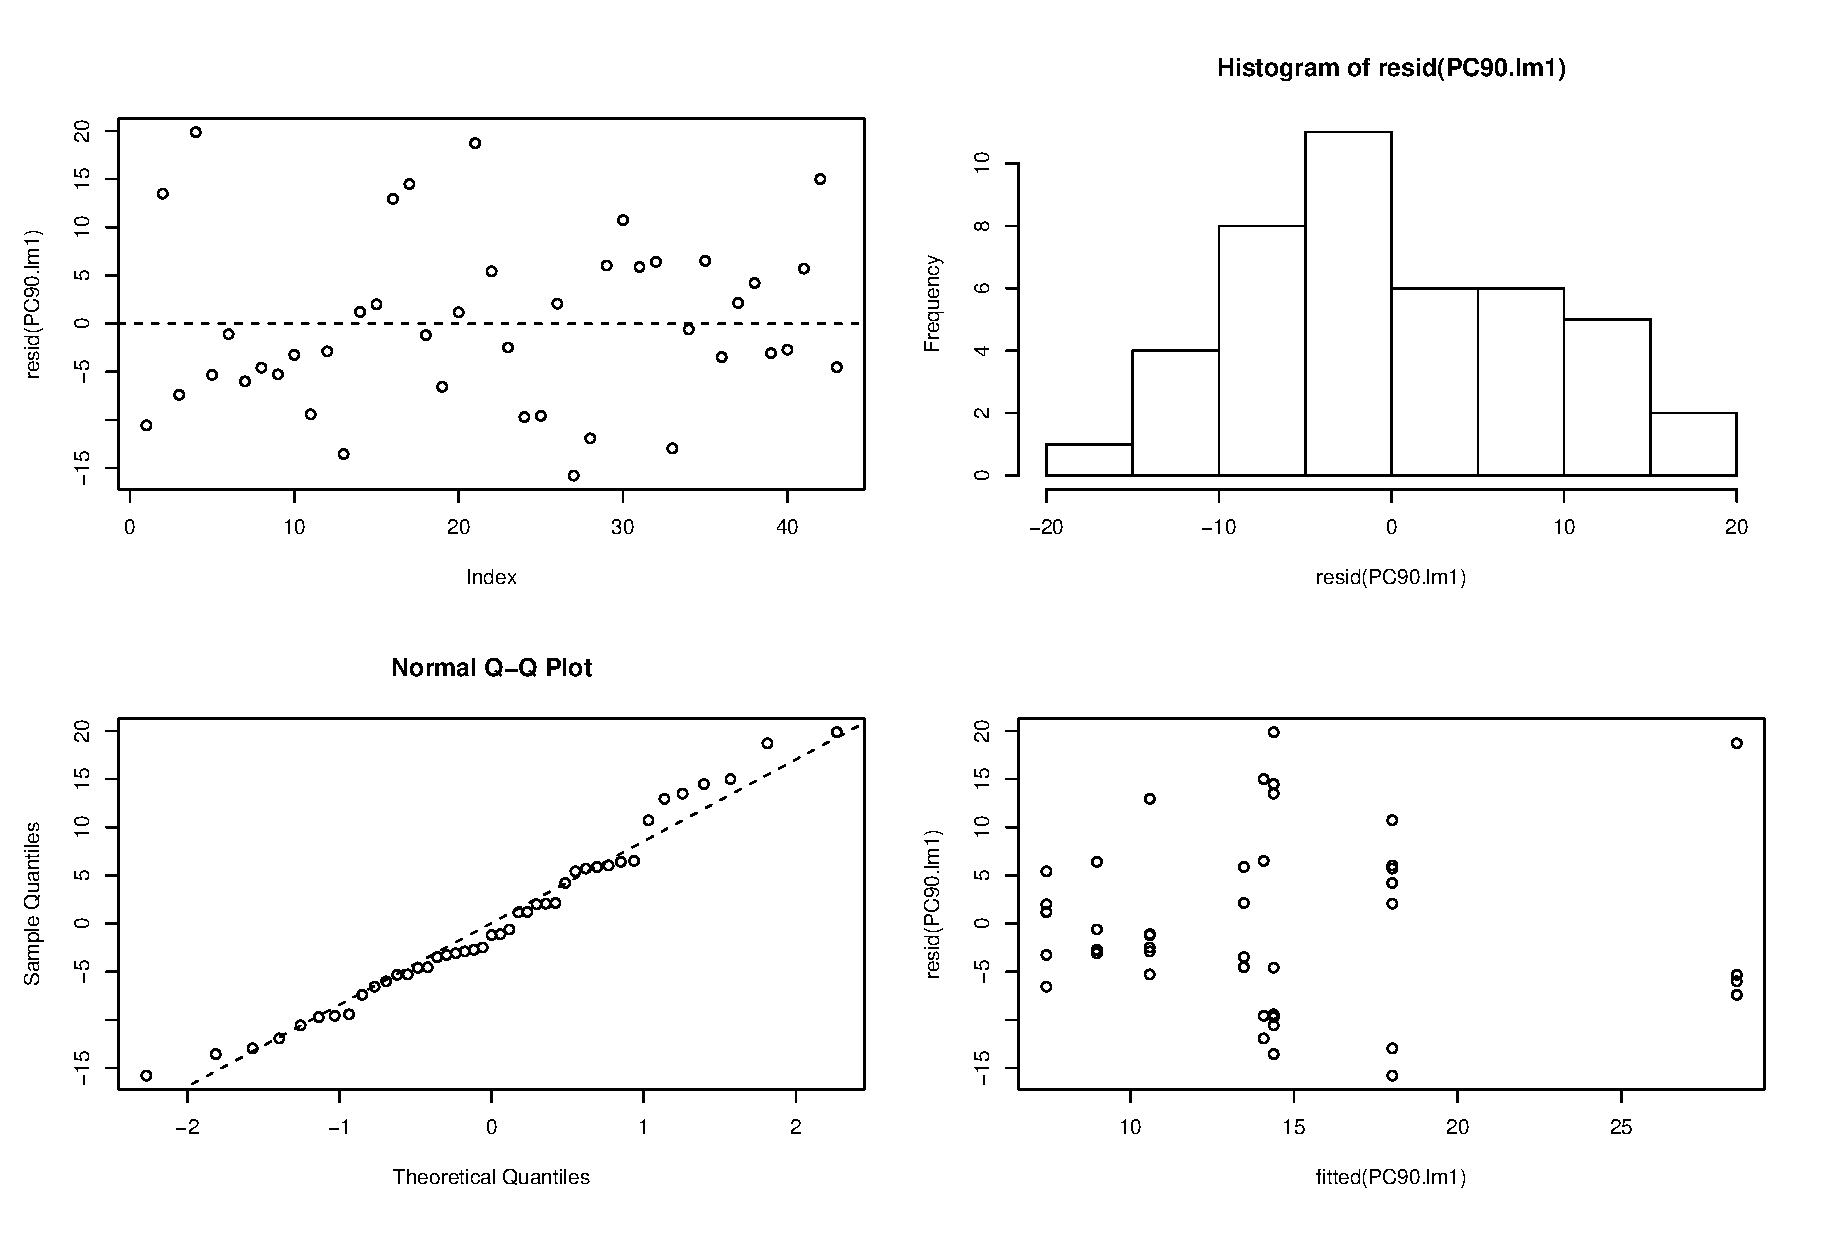
\includegraphics[scale=0.8]{PC90diag.eps}
\caption{Residuals for ANOVA on PC90}\label{resid}
\end{sidewaysfigure}
\section{Work Plan}
The next stages of the analysis are:
\begin{itemize}
\item Look in more detail at deriving the PC90 estimates. Logistic regression has been suggested in the project outline which would require non-linear regression techniques.
\item Look at how to identify and deal with suspicious outliers in the parasite count data and how they influence our estimates of PC90.
\item Incorporate the error in PC90 estimates into the modelling of treatment effect.
\end{itemize}

\section{Estimating PC90 for a patient}
\subsection{Cubic regression}
As described in the previous progress report a cubic model was fitted to the log-transformed parasite count $parct$ with time from first dose $t$ as the explanatory variable
$$log(1+parct)=\beta_0+\beta_1t+\beta_2t^2+\beta_3t^3+\epsilon\quad\quad\epsilon\sim N(0,\sigma^2)$$
The data was only fitted up to the first point that parasite count fell to 0 as the subsequent 0 count data is not relevant in determining the time to clearance. PC90 was then estimated from the fit by numerical optimisation with statistical software to find the value of $t$ corresponding to the point where the fitted model crosses a parasite count of $0.1P_0$, where $P_0$ is the initial pre-treatment parasite count.
\subsection{Logistic regression}
The logistic model fitted is
$$log(1+parct)=\alpha+\frac{\lambda}{1+e^{-\beta(t-\mu)}}+\epsilon$$
This was fitted to all the data as it can model a drop from an initial count level to a level of 0, unlike the cubic model. $\alpha$ is the lower asymptote which we would expect to be 0. $\alpha+\lambda$ is the upper asymptote which we would expect to be $P_0$. $\beta$ determines the rate of reduction with time and $\mu$ is the point of inflection (maximum rate of reduction). This model was fitted using non-linear least-squares routines in \emph{R} and \emph{SAS}.
\subsection{Interpolation}
The data points immediately above and below $0.1P_0$ were joined with a straight line fit and then the point where this line crosses $0.1P_0$ determines $t$ at PC90.

For loglinear interpolation the same procedure was performed only on a plot of $log(1+parct)$ vs. $t$.
\section{Comparison of results}
Figures \ref{1MB} and \ref{2FA} compare the logistic with the loglinear interpolation methods; the horizontal line is the PC90 level. It can be seen in Figure \ref{1MB} for Centre 1 male patients on treatment B that there is close agreement between the two methods. However in Figure \ref{2FA} for Centre 2 female patients on treatment A where the data is more ``erratic" that these simple approaches can fail in two ways.

Sometimes the non-linear fitting routine fails to converge on a solution (the plots with no logistic curve). This was found to be a problem using \texttt{nls} in \emph{R}. However, the \texttt{NLIN} routine in \emph{SAS} seems to achieve a reasonable solution in all cases. The second way in which this approach can fail is illustrated in the plot for patient 453 in Figure \ref{2FA} in that the parasite count temporarily dropped below the 10\% level before the actual final elimination of parasites had begun. It is clear that this approach should be modified to identify the \emph{last} time at which the parasite count drops below 10\%.

Table \ref{PC90} shows a comparison of the PC90 estimates by the four different methods looked at so far. Looking at the table the agreement in PC90 estimates looks fairly good. If we perform 6 paired-sample $t$-tests between pairs of methods we find that there is no strong evidence that the cubic regression and linear interpolation methods produce different estimates, likewise for the cubic and loglinear methods and the linear and logistic methods. The other combinations of methods do show evidence of difference in PC90 estimates ($P<0.0002$).

If we repeat the 3-way ANOVA of the previous report we find that \emph{Treatment} is the only factor that affects PC90 whichever method we use. Hence it would seem that the simplest method i.e. linear interpolation is the best method at this stage. However, as we know, the parasite count can be unreliable and depends on an operator-selected ``suitable" blood sample and so just one outlying value could throw the estimate by linear interpolation out as it only uses the two values above and below the PC90 count. In this respect an estimate based on more values should be more robust.
\begin{figure}
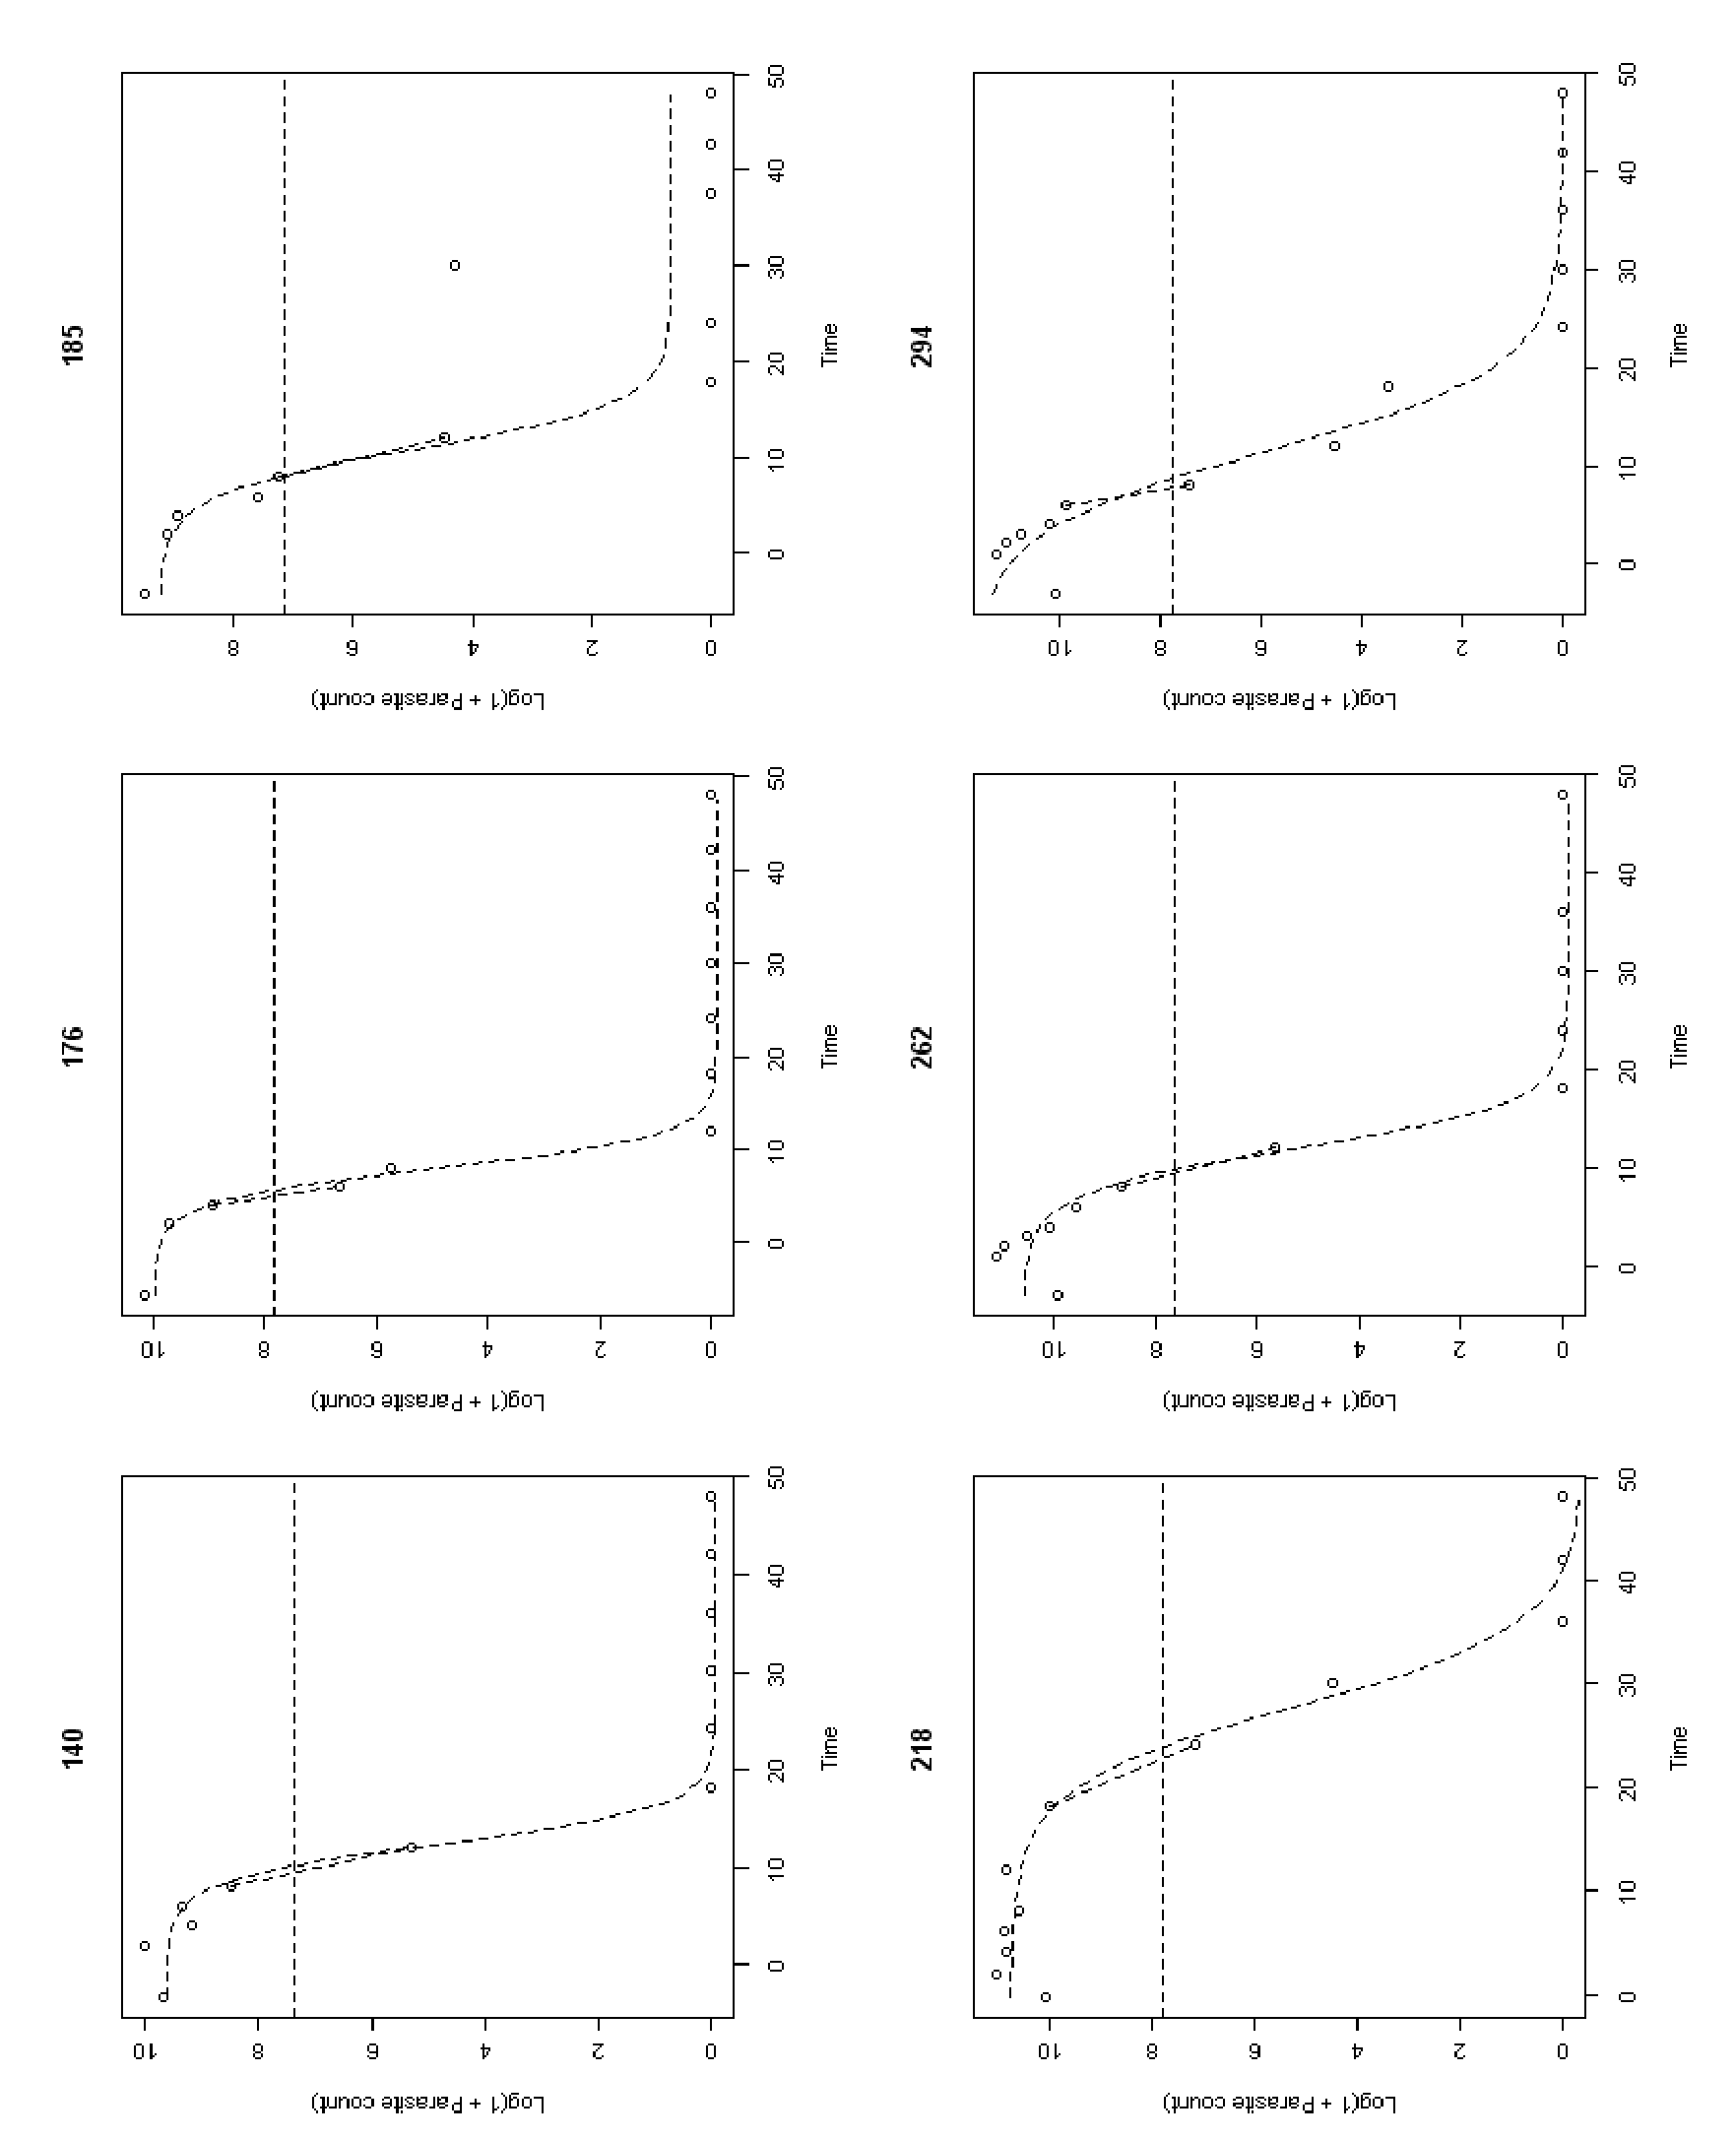
\includegraphics[scale=0.55]{logistic-1MB.eps} 
\caption{PC90 estimates for Centre 1 male patients on treatment B}\label{1MB}
\end{figure}
\begin{figure}
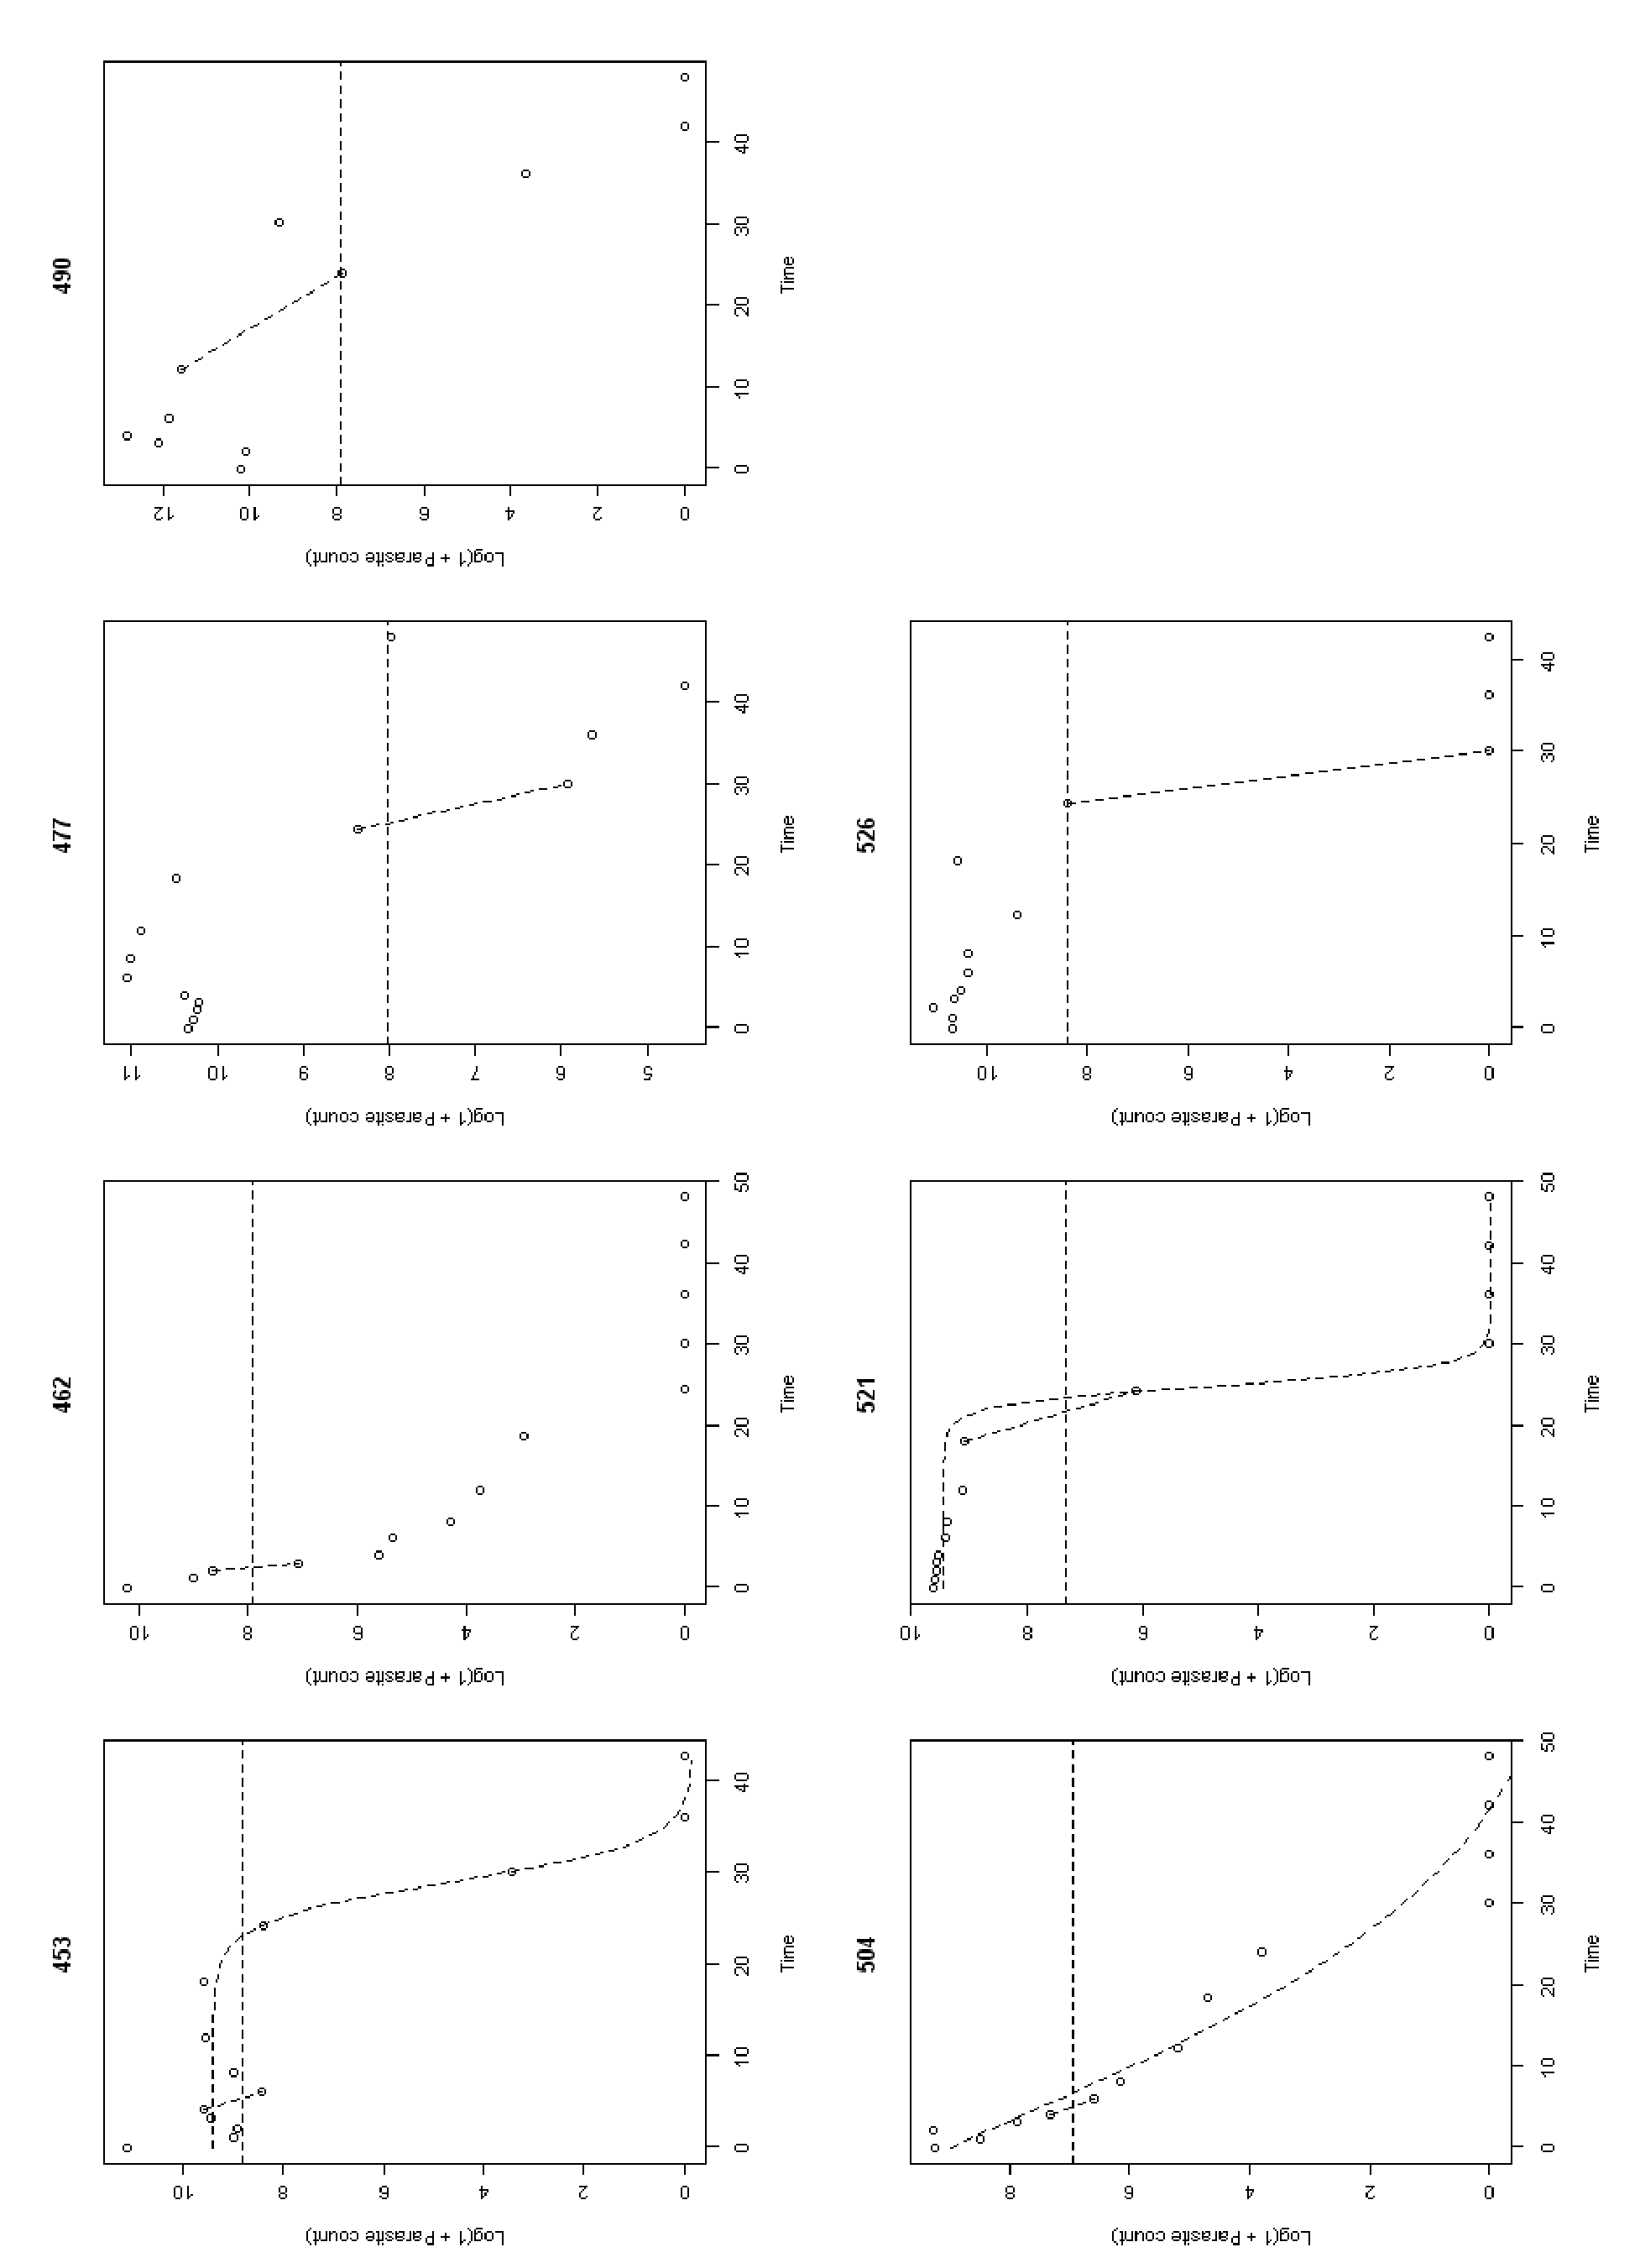
\includegraphics[scale=0.50]{logistic-2FA.eps} 
\caption{PC90 estimates for Centre 2 female patients on treatment A}\label{2FA}
\end{figure}
\begin{table}
\centering
\caption{Comparison of PC90 estimates by 4 methods}\label{PC90}
\begin{tabular}{|cccc|rrrr|}
\hline
Subject&Centre&&&PC90&PC90&PC90&PC90\\
ID&ID&Sex&Treatment&cubic&linear&loglinear&logistic\\
\hline
54&001&M&A&3.82&3.97&3.85&4.14\\
80&001&M&A&27.87&29.73&27.32&28.50\\
96&001&F&A&21.13&20.15&19.76&22.95\\
98&001&M&A&34.25&36.63&36.30&33.51\\
101&001&F&A&23.20&23.87&22.45&\\
140&001&M&B&9.49&10.90&9.46&10.16\\
150&001&F&A&22.53&23.24&21.75&23.12\\
162&001&M&A&9.79&9.10&8.84&\\
176&001&M&B&5.32&5.55&5.05&5.66\\
182&001&F&B&4.18&3.86&3.65&4.29\\
183&001&M&A&4.95&4.50&4.35&\\
185&001&M&B&7.70&8.33&8.09&8.13\\
187&001&M&A&0.83&1.93&1.53&3.05\\
197&001&F&B&8.64&9.87&8.15&8.35\\
203&001&F&B&9.44&11.27&9.69&10.30\\
218&001&M&B&23.54&23.76&22.77&23.92\\
224&001&M&A&28.86&30.02&30.01&30.26\\
262&001&M&B&9.40&10.74&9.40&9.85\\
264&001&F&B&0.88&0.96&0.85&1.43\\
280&001&F&B&8.61&9.92&9.04&9.72\\
285&001&F&A&47.24&46.76&46.52&\\
288&001&F&B&12.86&9.67&9.38&12.38\\
294&001&M&B&8.11&7.93&7.73&8.68\\
295&001&M&A&4.67&5.11&4.83&4.98\\
449&002&M&A&4.50&5.42&4.82&\\
453&002&F&A&20.07&22.73&21.97&23.08\\
462&002&F&A&2.22&2.67&2.49&\\
469&002&M&A&2.15&2.26&2.21&\\
477&002&F&A&24.03&26.10&25.08&\\
490&002&F&A&28.73&24.10&24.17&29.94\\
500&002&M&B&19.35&18.03&17.15&19.66\\
502&002&F&B&15.39&16.10&14.77&16.33\\
504&002&F&A&5.04&5.18&5.00&6.64\\
505&002&F&B&8.37&10.30&8.74&9.02\\
509&002&M&A&20.58&11.79&11.59&18.63\\
511&002&M&B&9.99&10.55&9.51&10.91\\
519&002&M&B&15.60&16.54&14.68&16.08\\
521&002&F&A&22.21&23.34&21.64&23.38\\
523&002&F&B&5.90&5.93&5.84&7.20\\
525&002&F&B&6.26&6.91&6.11&6.17\\
526&002&F&A&23.71&24.46&24.42&\\
530&002&M&A&29.07&29.53&28.09&29.28\\
532&002&M&B&8.94&8.33&8.08&9.21\\
\hline
\end{tabular}
\end{table}